\clearpage

\section{Discrete to continuous time}

This block converts a signal discrete in time to a signal continuous in time. It accepts one input signal that is a sequence of 1's and -1's and it produces one output signal that is a sequence of Dirac delta functions.

\subsection*{Input Parameters}

\begin{itemize}
	\item numberOfSamplesPerSymbol\{8\} \linebreak
	(int)
\end{itemize}

\subsection*{Methods}

DiscreteToContinuousTime(vector$<$Signal *$>$ \&inputSignals, vector$<$Signal *$>$ \&outputSignals) :Block(inputSignals, outputSignals)\{\};
\bigbreak	
void initialize(void);
\bigbreak	
bool runBlock(void);
\bigbreak	
void setNumberOfSamplesPerSymbol(int nSamplesPerSymbol)
\bigbreak
int const getNumberOfSamplesPerSymbol(void)

\subsection*{Functional Description}

This block reads the input signal buffer value, puts it in the output signal buffer and it fills the rest of the space available for that symbol with zeros. The space available in the buffer for each symbol is given by the parameter \textit{numberOfSamplesPerSymbol}.

\subsection*{Input Signals}

\subparagraph*{Number}: 1

\subparagraph*{Type}: Sequence of 1's and -1's. (DiscreteTimeDiscreteAmplitude)

\subsection*{Output Signals}

\subparagraph*{Number}: 1

\subparagraph*{Type}: Sequence of Dirac delta functions (ContinuousTimeDiscreteAmplitude)

\subsection*{Example}

\begin{figure}[h]
	\centering
	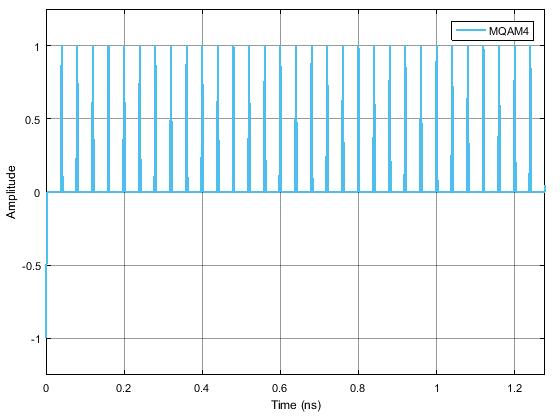
\includegraphics[width=\textwidth]{../m_qam_transmitter/figures/TimeDiscreteToContinuous_output}
	\label{MQAM4_DeterministicAppendZeros}\caption{Example of the type of signal generated by this block for a binary sequence 0100...}
\end{figure}

%\subsection*{Sugestions for future improvement}

\pagebreak
